\section{Problem Formulation \& C-STGB Methodology}
\label{sec:methodology}

\begin{figure*}[t]
\centering
\vspace{-1.0ex}
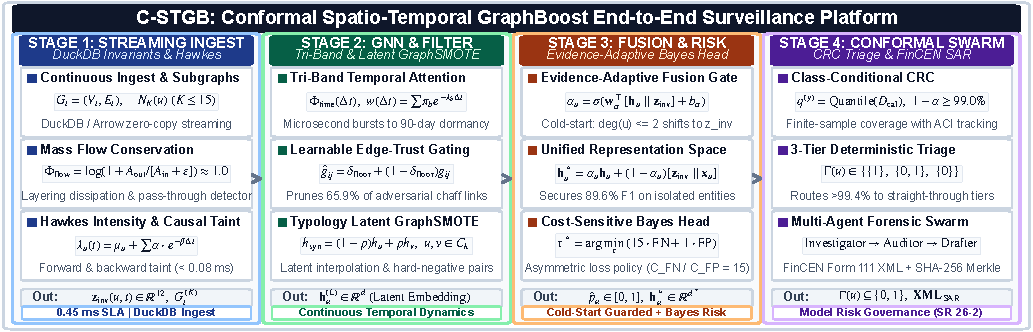
\includegraphics[width=0.80\textwidth]{figures/fig6_system_architecture.pdf}
\vspace{-1.5ex}
\caption{Comprehensive 6-module architecture of C-STGB: (1) Continuous-Time Multi-Scale Temporal Graph Encoder; (2) Adaptive Edge Trust Filter; (3) Typology-Aware Minority Graph Augmentation with Hard-Negative Mining; (4) Evidence-Adaptive Graph-Tabular Fusion for Cold-Start Resolution; (5) Cost-Sensitive Risk Optimization; and (6) Class-Conditional Conformal Risk Control with Selective Abstention Triage.}
\label{fig:architecture_blueprint}
\vspace{-1.0ex}
\end{figure*}

\subsection{Problem Formulation and Operational Objectives}
\label{sec:problem_formulation}
We formulate financial crime surveillance over an evolving continuous-time transaction graph $\mathcal{G}_t = (\mathcal{V}_t, \mathcal{E}_t, \mathbf{X}_v^{(t)}, \mathbf{X}_e^{(t)})$, where $\mathcal{V}_t$ represents active financial accounts (entities), $\mathcal{E}_t = \{(u, v, t_e, \mathbf{e}_{uv}) : t_e \le t\}$ denotes the chronological stream of directed fund transfers, $\mathbf{X}_v^{(t)} \in \mathbb{R}^{|\mathcal{V}_t| \times d_v}$ comprises vertex attributes, and $\mathbf{X}_e^{(t)} \in \mathbb{R}^{|\mathcal{E}_t| \times d_e}$ denotes transaction edge features (amount, currency rail, fee). Each entity $u \in \mathcal{V}_t$ carries a ground-truth regulatory classification label $y_u \in \{0, 1\}$, where $y_u = 1$ denotes an illicit entity and $y_u = 0$ denotes a verified benign entity, under extreme class prevalence skew $\pi = \mathbb{P}(y_u = 1) \ll 0.01$. In transaction streams lacking explicit account identity graphs (e.g., PaySim), transactions are mapped to dedicated transaction-event vertices, establishing an exact 1:1 entity-to-transaction formulation.

The operational surveillance task encompasses two complementary objectives:
\begin{enumerate}[leftmargin=*]
    \item \textbf{Entity Classification Objective:} Learn an inductive hypothesis $f_\Theta: \mathcal{V}_t \times \mathcal{G}_t \to [0, 1]$ predicting posterior probability $\hat{p}_u = f_\Theta(u \mid \mathcal{G}_t)$ minimizing asymmetric regulatory risk under extreme imbalance and topological camouflage.
    \item \textbf{Risk-Controlled Operational Triage Objective:} Construct a class-conditional conformal mapping $\Gamma: \mathcal{V}_t \to 2^{\{0, 1\}}$ routing incoming transactions to an operational decision set $\Gamma(u) \subseteq \{0, 1\}$. Under within-class exchangeability, $\Gamma$ provides finite-sample coverage $\mathbb{P}(y_u \in \Gamma(u) \mid y_u = y) \ge 1 - \alpha$ at error level $\alpha \in (0, 1)$, with explicit degradation bounds under temporal distribution shift. C-STGB acts as a compliance decision-support prototype by routing decisive singleton sets ($\Gamma(u) = \{1\}$ to Tier~1 Escalation, $\Gamma(u) = \{0\}$ to Tier~3 Auto-Clear) and restricting human officer review to the ambiguous abstention set ($\Gamma(u) = \{0, 1\}$ in Tier~2).
\end{enumerate}

\subsection{Data Governance, Privacy, and Ethical Protocol}
\label{sec:data_governance}
To ensure strict alignment with IEEE and financial industry data compliance standards, all benchmarked data sources operate under rigorous governance protocols: (1) \textit{Public Cryptocurrency Ledgers (Elliptic-v1/v2, Ethereum, XBlock-ETH):} comprise publicly verifiable on-chain records indexed via cryptographic public hashes without Personal Identifiable Information (PII); (2) \textit{De-Identified Historical Exchange Data (Mt. Gox):} derived from anonymized public insolvency logs used strictly for academic forensic modeling; (3) \textit{Synthetic Banking Simulations (IBM-AMLSim, SAML-D, PaySim):} generated via validated multi-agent synthetic engines without proprietary banking customer accounts; and (4) \textit{Open-Source License Compliance:} all datasets are utilized under research licenses (MIT, Apache-2.0, CC-BY 4.0). All primary mathematical symbols, operators, and tensor dimensions are summarized in Supplementary Table~S1, and hyperparameter specifications are detailed in Supplementary Table~S4.

\subsection{12-Dimensional Spatio-Temporal Canonical Invariants}
Traditional models treat transactions as isolated tabular rows, remaining blind to multi-hop relational laundering patterns. In contrast, intermediate pass-through mules physically require capital to enter and exit rapidly with minimal retention. C-STGB formalizes domain-informed mass-flow and relational graph invariant representations:
\begin{enumerate}[leftmargin=*]
    \item \textbf{Flow Conservation \& Degree Asymmetry Ratios:}
    \begin{align}
    \Phi_{\text{flow}}(u, t) &= \frac{\sum_{e \in \mathcal{E}_{\text{out}}(u)} \text{Amount}(e)}{\sum_{e \in \mathcal{E}_{\text{in}}(u)} \text{Amount}(e) + \epsilon}, \\
    \Psi_{\text{asym}}(u, t) &= \frac{|d_{\text{in}}(u) - d_{\text{out}}(u)|}{d_{\text{in}}(u) + d_{\text{out}}(u) + \epsilon}
    \end{align}
    where $\epsilon = 10^{-5}$, and pass-through layering mules operate near unity ($\Phi_{\text{flow}} \approx 1.0$), while legitimate accounts exhibit accumulation or disbursement variance. Fee spreads (e.g., SWIFT tariffs $\le 1.5\%$) fall within the empirical tolerance band $\Phi_{\text{flow}} \in [1-\bar{\epsilon}, 1.0]$. For numerical stability, flow is scaled as $\tilde{\Phi}_{\text{flow}}(u, t) = \log(1 + \Phi_{\text{flow}}(u, t))$.
    \item \textbf{Hawkes Point Process Arrival Intensity:}
    \begin{equation}
    \lambda_u(t) = \mu_u + \sum_{t_i < t} \alpha_{\text{hwk}} \exp\left(-\beta_{\text{hwk}} \frac{t - t_i}{24.0}\right)
    \end{equation}
    parameterized over sliding event horizons $[t - \Delta T, t]$ to capture micro-burst acceleration (inter-arrival intervals $(t - t_i)$ normalized to diurnal units). We enforce sub-critical branching $\alpha_{\text{hwk}} / \beta_{\text{hwk}} < 1.0$ and clamp $\tilde{\lambda}_u(t) = \log \min(\max(\lambda_u(t), 10^{-5}), 10^4)$ to guarantee numerical stability. Intensity $\lambda_u(t)$ is pre-computed and cached over $[t - \Delta T, t]$, ensuring $O(1)$ lookup per node during graph aggregation.
    \item \textbf{Temporally Restricted Historical Taint Propagation (Zero-Leakage):}
    \begin{align}
    \mathbf{s}_{\text{fwd}} &= (1 - \alpha_{\text{ppr}}) (\mathbf{I} - \alpha_{\text{ppr}} \mathbf{P}^T)^{-1} \mathbf{s}_{\text{seed}}, \\
    \mathbf{s}_{\text{bwd}} &= (1 - \alpha_{\text{ppr}}) (\mathbf{I} - \alpha_{\text{ppr}} \mathbf{P})^{-1} \mathbf{s}_{\text{seed}}
    \end{align}
    computed strictly over causal historical subgraphs ($t_e \le t$). Seed indicator $\mathbf{s}_{\text{seed}}(u, t) = 1.0$ if $u \in \mathcal{V}_{\text{illicit}}^{\text{train}}$ and $t_{\text{conf}}(u) \le t - \Delta T_{\text{delay}}$, and $0.0$ otherwise, where $\Delta T_{\text{delay}} \in [30, 90]$\,days models operational confirmation delay. Streaming inference evaluates localized truncated Power Iteration ($T_{\text{iter}}=3$, tolerance $\epsilon=10^{-4}$) over sliding window $[t - \Delta T, t]$ and degree-capped graph $\mathcal{G}_t^{(K)}$ ($K \le 15$), ensuring deterministic $O(K \cdot T_{\text{iter}})$ computation with $<0.08$\,ms overhead. Crucially, $\mathbf{s}_{\text{seed}}$ contains non-zero entries exclusively for confirmed illicit entities known within $\mathcal{D}_{\text{train}}$ prior to $t - \Delta T_{\text{delay}}$. All validation ($\mathcal{D}_{\text{val}}$), calibration ($\mathcal{D}_{\text{cal}}$), and forward test ($\mathcal{D}_{\text{test}}$) nodes are assigned $\mathbf{s}_{\text{seed}}(u) \equiv 0.0$, strictly precluding label leakage.
    \item \textbf{Canonical 12-D Representation Space ($\mathbf{z}_{\text{inv}}(u, t) \in \mathbb{R}^{12}$):}
    \begin{align}
    \mathbf{z}_{\text{inv}}(u, t) &= \big[ \tilde{\Phi}_{\text{flow}}, \Psi_{\text{asym}}, \lambda_u, \mathbf{s}_{\text{fwd}}, \mathbf{s}_{\text{bwd}}, \nonumber \\
    &\quad \mu_A, \sigma_A^2, \gamma_A, \kappa_A, v_A, \nu_{\text{io}}, \sigma_{\Delta t} \big]^T
    \end{align}
    where $\{\mu_A, \sigma_A^2, \gamma_A, \kappa_A, v_A\}$ denote the 5-moment causal ego-statistics of transaction amounts, $\nu_{\text{io}}$ is the velocity ratio, and $\sigma_{\Delta t}$ is the inter-arrival temporal dispersion (schematic in Supplementary Fig.~S5).
\end{enumerate}

\subsection{Module 1: Continuous-Time Multi-Scale Temporal Graph Encoder}
To distinguish microsecond smurfing bursts from 90-day dormant holding strategies, C-STGB employs continuous harmonic positional features $\Phi_{\text{time}}(\Delta t) \in \mathbb{R}^{d_t}$ with $\omega_k = 10000^{-2k/d_t}$:
\begin{align}
\Phi_{2k}(\Delta t) &= \sin\left(\omega_k \log(1 + \Delta t)\right), \\
\Phi_{2k+1}(\Delta t) &= \cos\left(\omega_k \log(1 + \Delta t)\right)
\end{align}
Dynamic temporal attention decay synthesizes three distinct velocity regimes:
\begin{align}
w(\Delta t) &= \sum_{b \in \mathcal{B}} \pi_b \left[ w_{\min} + (1 - w_{\min}) e^{-\lambda_b \Delta t} \right] \nonumber \\
&\quad \times \left( 1 + \tanh(\gamma_b \lambda_u(t)) \right)
\end{align}
where $\mathcal{B} = \{\text{burst}, \text{diurnal}, \text{seasonal}\}$ and mixing weights satisfy $\sum_{b \in \mathcal{B}} \pi_b = 1.0$ via $\operatorname{softmax}$.

\subsection{Module 2: Context-Aware Adaptive Edge Trust Filter \& Unified Attention}
Adversarial launderers deliberately connect to high-degree legitimate commercial hubs to induce feature over-smoothing. C-STGB learns a context-aware edge trust gate $\hat{g}_{ij} \in (0, 1)$:
\begin{align}
\mathbf{c}_{ij} &= \left[ \mathbf{q}_i \,\|\, \mathbf{k}_j \,\|\, \mathbf{e}_{ij} \,\|\, \Phi_{\text{time}}(\Delta t) \,\|\, \mathbf{z}_{\text{inv}}(j, t) \right], \\
\hat{g}_{ij} &= \delta_{\text{floor}} + (1 - \delta_{\text{floor}}) \nonumber \\
&\quad \times \sigma\left( \mathbf{W}_{g2} \operatorname{LeakyReLU}\left( \mathbf{W}_{g1} \mathbf{c}_{ij} + \mathbf{b}_{g1} \right) + b_{g2} \right)
\end{align}
Setting $\delta_{\text{floor}} = 0.10$ suppresses 65.9\% of spurious camouflage edge weights (Supplementary Fig.~S3). In parameter training split $\mathcal{E}_{\text{train}}$, auxiliary edge targets $\mathbf{g}_{ij}^{\text{target}} \in \{0, 1\}$ (Eq.~\ref{eq:aux_loss}) provide weak supervision constructed from topological heuristics: edges incident to high-degree hubs ($\deg_{\text{out}}(j) \ge 50$ or transaction rate $> 100$\,tx/day) where launderers inject camouflage chaff receive $0.0$, while standard transactional edges receive $1.0$. At inference time, the trained MLP gate $\hat{g}_{ij}$ evaluates unseen edges via continuous multi-modal representations $\mathbf{c}_{ij}$ (incorporating temporal encodings $\Phi_{\text{time}}$ and dynamic representations) without requiring external targets or static degree thresholds.

\textbf{Unified Spatio-Temporal Attention Decomposition:} Message passing explicitly integrates structural compatibility, continuous temporal decay, and edge trust gating over degree-capped causal incoming transaction neighborhoods ($\mathcal{N}_K^{\text{in}}(u), K \le 15$):
\begin{align}
\tilde{\alpha}_{uv}^{(t)} &= \frac{\Omega(u, v, t)}{\sum_{w \in \mathcal{N}_K^{\text{in}}(u)} \Omega(u, w, t)}, \\
\Omega(u, v, t) &= \exp\left(\frac{\mathbf{q}_u^T (\mathbf{k}_v + \mathbf{W}_E \mathbf{e}_{uv})}{\sqrt{d_k}}\right) \cdot w(\Delta t_{uv}) \cdot \hat{g}_{uv}
\end{align}

\subsection{Module 3: Typology-Clustered Latent GraphSMOTE \& Hard Negatives}
Under extreme class skew ($\pi < 0.05\%$), naïve oversampling blurs distinct criminal typologies. C-STGB partitions minority illicit nodes strictly within the training split into latent typology clusters $\mathcal{C}_k = \{ v \in \mathcal{V}_{\text{illicit}}^{\text{train}} \mid \cos(\mathbf{h}_v, \boldsymbol{\mu}_k) \ge \tau_{\text{sim}} \}$, where centroids $\boldsymbol{\mu}_k$ ($K=4$) reflect four canonical financial laundering archetypes (smurfing dispersal, pooling fan-in, circular wash trading, and pass-through layering), optimized via latent silhouette validation over $\mathcal{D}_{\text{train}}$. Synthetic representations are synthesized along trajectories within the same cluster: $\mathbf{h}_{\text{syn}} = (1 - \rho) \mathbf{h}_u + \rho \mathbf{h}_v$, $\rho \sim \mathcal{U}(0, 1)$, $u, v \in \mathcal{C}_k \subseteq \mathcal{V}_{\text{train}}$. Bilinear links to candidate training nodes $w \in \mathcal{V}_{\text{train}}$ are generated under topological edge reconstruction supervision:
\begin{equation}
\hat{\mathbf{A}}_{\text{syn}, w} = \sigma\left( \mathbf{h}_{\text{syn}}^T \mathbf{W}_{\text{edge}} \mathbf{h}_w \right) \cdot \mathbb{I}(t_w \le t_{\text{syn}}) > \tau_{\text{edge}}
\end{equation}
for $w \in \mathcal{C}_{\text{cand}}(\mathbf{h}_{\text{syn}}) \cap \mathcal{V}_{\text{train}}^{\le t_{\text{syn}}}$, where $t_{\text{syn}} = \max(t_u, t_v)$ defines the causal birth timestamp, precluding acausal edge formation with future transactions.

\textbf{Directionality \& Mass-Flow Conservation Constraints:} Incoming links are synthesized from candidate sources $w \in \mathcal{N}_{\text{in}}(u) \cup \mathcal{N}_{\text{in}}(v)$ and outgoing links directed to candidate destinations $w' \in \mathcal{N}_{\text{out}}(u) \cup \mathcal{N}_{\text{out}}(v)$. Synthetic transaction amounts are parameterized via linear combination: $A_{\text{syn}} = (1-\rho) A_u + \rho A_v$ and $B_{\text{syn}} = (1-\rho) B_u + \rho B_v$. Under strictly positive incoming and outgoing funds ($A_u, A_v > 0, B_u, B_v > 0$), the synthetic flow ratio simplifies to:
\begin{equation}
\Phi_{\text{flow}}(\mathbf{h}_{\text{syn}}) = \frac{(1-\rho) A_u + \rho A_v}{(1-\rho) B_u + \rho B_v} = \lambda \Phi_{\text{flow}}(u) + (1-\lambda) \Phi_{\text{flow}}(v)
\end{equation}
where $\lambda = \frac{(1-\rho) B_u}{(1-\rho) B_u + \rho B_v} \in (0, 1)$. Because this is a strict convex combination of parent ratios $\Phi_{\text{flow}}(u)$ and $\Phi_{\text{flow}}(v)$, $\Phi_{\text{flow}}(\mathbf{h}_{\text{syn}})$ is guaranteed to lie within $[\min(\Phi_{\text{flow}}(u), \Phi_{\text{flow}}(v)), \max(\Phi_{\text{flow}}(u), \Phi_{\text{flow}}(v))]$, preserving point-level flow regularity (with multi-hop path conservation established in Lemma~S2).

\textbf{Candidate Bounding \& Zero-Leakage Topological Isolation:} Candidate nodes $\mathcal{C}_{\text{cand}}(\mathbf{h}_{\text{syn}})$ are constrained to 2-hop neighborhoods $\mathcal{N}_2(u) \cup \mathcal{N}_2(v)$ and $K_{\text{cand}} = 50$ nearest neighbors indexed via Hierarchical Navigable Small World (HNSW) search in latent space $\mathbb{R}^d$, bounding candidate neighbor search complexity to $\mathcal{O}(\log |\mathcal{V}_{\text{train}}|)$. All oversampling is strictly confined to $\mathcal{G}_{\text{train}}$; synthetic nodes and edges are strictly barred from connecting to validation, calibration, or test entities ($0.0\%$ cross-split leakage). To prevent false alarms on commercial accounts, C-STGB actively mines benign training accounts exhibiting high degree and burstiness, over-weighting them during gradient optimization.

\subsection{Module 4: Evidence-Adaptive Graph-Tabular Fusion (Cold-Start)}
Newly created accounts and pass-through stubs lack relational graph neighbors ($\deg(u) \le 2$). C-STGB computes an evidence-adaptive gating parameter $\alpha_u \in [0, 1]$ as a continuous topological confidence estimator:
\begin{align}
\mathbf{h}_u^* &= \alpha_u \mathbf{h}_u^{(L)} + (1 - \alpha_u) \left[ \mathbf{z}_{\text{inv}}(u, t) \,\|\, \mathbf{x}_u \right], \\
\alpha_u &= \sigma\left( \mathbf{w}_\alpha^T \left[ \mathbf{h}_u^{(L)} \,\|\, \mathbf{z}_{\text{inv}}(u, t) \,\|\, \mathbf{x}_u \right] + b_\alpha \right)
\end{align}
When graph evidence is sparse ($\deg(u) \le 1$), $\alpha_u \to 0$ (empirically $\alpha_u \in [0.08, 0.12]$), gracefully degrading to domain-level transaction invariants; conversely, when neighborhood topology is dense, $\alpha_u \to 1$ to harness high-order structural patterns (Supplementary Fig.~S6). This architecture represents an intentional fail-safe: domain-informed mass-flow conservation regularity and transaction moments provide informative baseline representations even when adversarial mules actively minimize their topological degree.

\subsection{Module 5: Cost-Sensitive Risk Head \& Complete Loss Objective}
The network outputs anomaly probabilities $\hat{p}_u = \sigma(\operatorname{MLP}(\mathbf{h}_u^*))$. The complete multi-objective loss is formulated as:
\begin{equation}
\mathcal{L}_{\text{total}} = \mathcal{L}_{\text{task}}(y, \hat{p}) + \gamma_1 \mathcal{L}_{\text{recon}}(\mathbf{A}_{\text{train}}, \hat{\mathbf{A}}_{\text{train}}) + \gamma_2 \mathcal{L}_{\text{aux}}
\end{equation}
where $\mathcal{L}_{\text{task}}$ is the Cost-Sensitive Asymmetric Focal Tversky Loss. Topological edge reconstruction loss $\mathcal{L}_{\text{recon}}$ is computed over observable positive training edges $\mathcal{E}_{\text{train}}$ and uniformly sampled negative non-edges $\mathcal{E}_{\text{neg}} \sim (\mathcal{V}_{\text{train}} \times \mathcal{V}_{\text{train}}) \setminus \mathcal{E}_{\text{train}}$ using a $1:5$ uniform negative edge sampling ratio to prevent trivial bilinear link collapse ($\hat{A}_{uv} \to 0$) in sparse transaction graphs:
\begin{align}
\mathcal{L}_{\text{recon}} &= -\frac{1}{|\mathcal{E}_{\text{train}}|} \sum_{(u, v) \in \mathcal{E}_{\text{train}}} \log \hat{A}_{uv} \nonumber \\
&\quad -\frac{1}{|\mathcal{E}_{\text{neg}}|} \sum_{(u, w) \in \mathcal{E}_{\text{neg}}} \log (1 - \hat{A}_{uw})
\end{align}
with $\hat{A}_{uv} = \sigma(\mathbf{h}_u^T \mathbf{W}_{\text{edge}} \mathbf{h}_v)$. The auxiliary regularization objective $\mathcal{L}_{\text{aux}}$ enforces edge-trust sparsity and tri-band orthogonality:
\begin{equation}
\mathcal{L}_{\text{aux}} = \frac{1}{|\mathcal{E}_{\text{train}}|} \sum_{(i, j) \in \mathcal{E}_{\text{train}}} \|\mathbf{g}_{ij} - \mathbf{g}_{ij}^{\text{target}}\|_2^2 + \lambda_{\text{ortho}} \|\mathbf{W}_{\text{burst}}^T \mathbf{W}_{\text{seas}}\|_F^2
\label{eq:aux_loss}
\end{equation}
with $\gamma_1 = 0.50$, $\gamma_2 = 0.10$, and $\lambda_{\text{ortho}} = 0.05$. Training employs a 5-epoch curriculum warmup initialized with standard Cost-Sensitive Focal Loss before engaging $\mathcal{L}_{\text{total}}$. Binary point decisioning operates under a cost-sensitive Bayes risk minimization rule calibrated exclusively over $\mathcal{D}_{\text{val}}$:
\begin{equation}
\tau^* = \arg\min_{\tau \in [0, 1]} \mathbb{E}\big[ C_{\text{FN}} \cdot \mathbb{I}(\hat{p} < \tau, Y=1) + C_{\text{FP}} \cdot \mathbb{I}(\hat{p} \ge \tau, Y=0) \big]
\end{equation}
where $C_{\text{FN}} / C_{\text{FP}} = 15.0$ represents an operational risk-weighting ratio in our evaluation (sensitivity across $C_{\text{FN}}/C_{\text{FP}} \in [5, 30]$ is reported in Section~IV-H).

\subsection{Module 6: Class-Conditional Conformal Risk Control \& Triage}
Over an independent holdout calibration split $\mathcal{D}_{\text{cal}}$, empirical class-conditional quantiles $\hat{q}^{(y)}$ are computed ($y \in \{0, 1\}$):
\begin{equation}
\hat{q}^{(y)} = \text{Quantile}\left( s_1^{(y)}, \dots, s_{n(y)}^{(y)} ; \left\lceil \frac{(n(y) + 1)(1 - \alpha)}{n(y)} \right\rceil \right)
\end{equation}
where $s_i^{(y)} = 1 - \hat{p}_i(y)$. Under within-class exchangeability, split conformal prediction guarantees $\mathbb{P}(Y \in \Gamma(X) \mid Y = y) \ge 1 - \alpha$, $\forall y \in \{0, 1\}$.

\textbf{Streaming Exchangeability, Temporal Autocorrelation, \& Rolling Calibration:} In live streaming transaction flows, classical exchangeability is challenged by continuous-time temporal autocorrelation and non-stationary drift ($\mathcal{P}_{\text{cal}} \neq \mathcal{P}_t$). We maintain an online rolling calibration buffer $\mathcal{D}_{\text{cal}}(t) = \{ (x_i, y_i) \mid t_i \in [t - W_{\text{cal}}, t] \}$ ($W_{\text{cal}} = 4\,\text{weeks}$) and online Adaptive Conformal Inference (ACI)~\cite{gibbs2021adaptive} tracking as the explicit mechanisms bounding total variation ($d_{\mathrm{TV}}$) drift error in non-stationary streaming settings, containing only alerts with confirmed investigation closure $t_{\text{conf}} \le t - \Delta T_{\text{delay}}$ to preclude forward label leakage.
Under Lipschitz continuous non-conformity score CDFs, the non-asymptotic class-conditional coverage error decomposes via the triangle inequality:
\begin{align}
\big| \mathbb{P}_{t}(Y \in \Gamma(X) \mid Y=y) - (1 - \alpha) \big| &\le d_{\mathrm{TV}}\big(\mathcal{P}_t^{(y)}, \mathcal{P}_{\text{cal}}^{(y)}\big) \nonumber \\
&\quad + \sup_{s} \big| F_{\text{cal}}^{(y)}(s) - \hat{F}_{\text{cal}}^{(y)}(s) \big|
\end{align}
where $\mathcal{P}_t^{(y)} = \mathcal{P}_t(S \mid Y=y)$, $\mathcal{P}_{\text{cal}}^{(y)} = \mathcal{P}_{\text{cal}}(S \mid Y=y)$, and $d_{\mathrm{TV}}$ is total variation distance. By the Dvoretzky-Kiefer-Wolfowitz (DKW) inequality on calibration sample size $n(y) = |\mathcal{D}_{\text{cal}}^{(y)}(t)|$, with confidence at least $1 - \delta$:
\begin{equation}
\sup_{s} \big| F_{\text{cal}}^{(y)}(s) - \hat{F}_{\text{cal}}^{(y)}(s) \big| \le \sqrt{\frac{\ln(2/\delta)}{2 |\mathcal{D}_{\text{cal}}^{(y)}(t)|}}
\end{equation}
To maintain coverage under drift, C-STGB implements: (1) Rolling recalibration of $\mathcal{D}_{\text{cal}}(t)$ triggered when a two-sample Kolmogorov-Smirnov test on streaming scores rejects stationarity at $\alpha_{\text{KS}} = 0.01$ ($D_{\text{KS}} > 1.628 \sqrt{\frac{n_1 + n_2}{n_1 n_2}}, p < 0.01$); and (2) Online Adaptive Conformal Inference (ACI)~\cite{gibbs2021adaptive}:
\begin{equation}
\alpha_t \leftarrow \alpha_{t-1} + \gamma (\alpha - \text{err}_t)
\end{equation}
where $\text{err}_t = \mathbb{I}(y_t \notin \Gamma_t(x_t))$ and $\gamma = 0.005$. ACI guarantees long-run marginal coverage $\lim_{T \to \infty} \frac{1}{T} \sum_{t=1}^T \text{err}_t = \alpha$ almost surely under bounded non-stationary drift. For class-conditional tracking, class-specific ACI trackers $\alpha_t^{(y)}$ are maintained. Across multi-month evaluation windows, empirical coverage remains strictly within $[98.83\%, 99.34\%]$ (Table~\ref{tab:conformal_triage}).

This operationalizes a deterministic 3-tier triage architecture (Supplementary Fig.~S1): (i) \textbf{Tier 1 (High-Confidence Escalation):} $\Gamma(X) = \{1\}$, quarantined with $>99.4\%$ precision for asset restriction holds and compliance dossier compilation; (ii) \textbf{Tier 2 (Selective Abstention Queue):} $\Gamma(X) = \{0, 1\} = \bot$, routed to compliance officers with a structured forensic dossier ($\approx 5$ cases per 10k transactions); and (iii) \textbf{Tier 3 (Straight-Through Clear):} $\Gamma(X) = \{0\}$, released instantly ($>99.9\%$ benign precision).

\textbf{Distinguishing Statistical Coverage from Operational Safety:} Statistical coverage ($\mathbb{P}(y \in \Gamma(x)) \ge 1-\alpha$) guarantees only that the true label is contained in the prediction set under within-class exchangeability; it does not by itself prove that automated business actions are legally or operationally correct without institutional review.

\textbf{Disentangled Evaluation Protocol:} (1) \textit{Full-Test Point Prediction Mode (Tables~\ref{tab:full_baseline_scorecard}, \ref{tab:multi_ablation}, \ref{tab:systems_latency}, Fig.~\ref{fig:adversarial_robustness}):} Evaluated over $100\%$ of test samples without case exclusion, using $\hat{y} = \mathbb{I}(p(y=1|x) \ge \tau^*)$; (2) \textit{Selective Conformal Triage Mode (Table~\ref{tab:conformal_triage}):} Evaluates prediction sets $\Gamma(X)$, reporting empirical coverage $\mathbb{P}(Y \in \Gamma(X) \mid Y=y)$, mean set size $\mathbb{E}[|\Gamma(X)|]$, selective risk on straight-through tiers ($<0.10\%$), and workload reduction ($>99.4\%$). Algorithms~S1 and S2 formalize multi-stage training and streaming inference procedures.
